% Part: sets-functions-relations
% Chapter: relations
% Section: graphs

\documentclass[../../../include/open-logic-section]{subfiles}

\begin{document}

\olfileid{sfr}{rel}{grp}
\olsection{Grafen}

Een \emph{graaf} is een diagram waarin punten---‘knopen’ of
‘knooppunten’ genoemd (het meervoud van ‘knooppunt’)---door lijnen met
elkaar zijn verbonden. Grafen worden overal in de discrete wiskunde
en informatica gebruikt. Ze zijn bijzonder geschikt om relaties en
structuren weer te geven en in beeld te brengen, van concrete zaken
zoals allerlei soorten netwerken tot abstracte structuren zoals de
mogelijke uitkomsten van beslissingen. In de literatuur komen veel
soorten grafen voor. Ze verschillen er bijvoorbeeld in of hun
lijnen gericht zijn, of ze labels dragen, of een lijn van een knoop
naar diezelfde knoop mag lopen en of dezelfde knopen door meerdere
lijnen verbonden mogen zijn. \emph{Gerichte grafen} houden op een
bijzondere manier verband met relaties.

\begin{defn}[Gerichte graaf]
Een \emph{gerichte graaf} $G = \tuple{V, E}$ bestaat uit een
verzameling \emph{knopen}~$V$ en een verzameling
\emph{pijlen}~$E \subseteq V^2$.
\end{defn}

\begin{explain}
Volgens deze definitie is een graaf niets anders dan een verzameling
met daarop een relatie. Bij een graaf ligt een tekening uiteraard voor
de hand: we tekenen precies dan een pijl van knoop~$v_1$ naar knoop
$v_2$ als $\tuple{v_1, v_2} \in E$. Het enige verschil tussen een
relatie en een graaf is dat een graaf, anders dan de relatie alleen,
ook de verzameling knopen vermeldt; een graaf kan dus geïsoleerde
knopen hebben. Van
belang is echter dat elke relatie~$R$ op een verzameling~$X$ kan
worden opgevat als de gerichte graaf $\tuple{X, R}$. Omgekeerd kan een
gerichte graaf~$\tuple{V, E}$ worden opgevat als een relatie
$E \subseteq V^2$, waarbij de verzameling $V$ uitdrukkelijk is
vermeld.
\end{explain}

\begin{ex}
De graaf $\tuple{V, E}$ met $V = \{1, 2, 3, 4\}$ en $E =
\{\tuple{1,1}, \allowbreak \tuple{1, 2}, \allowbreak \tuple{1, 3},
\allowbreak \tuple{2, 3}\}$ ziet er als volgt uit:
\begin{align*}
& 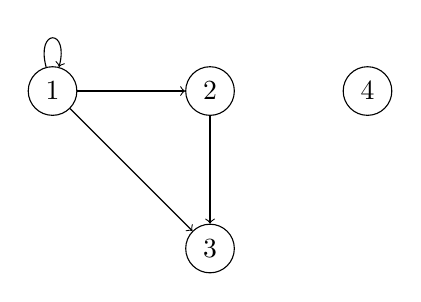
\begin{tikzpicture}[->,node distance=2cm]
  \node[draw,circle] (A) {$1$};
  \node[draw,circle] (B) [right of=A] {$2$};
  \node[draw,circle] (C) [below of=B] {$3$};
  \node[draw,circle] (D) [right of=B] {$4$};
  \draw (A) to [loop above]  (A);
  \draw (A) to  (B);
  \draw (A) to  (C);
  \draw (B) to  (C);
  \end{tikzpicture}
\intertext{Dit is een andere graaf dan $\tuple{V', E}$ met $V' =
  \{1, 2, 3\}$, die er als volgt uitziet:}
& 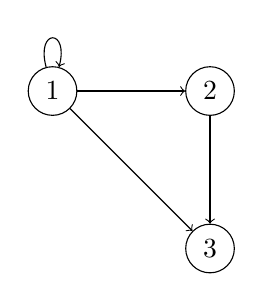
\begin{tikzpicture}[->,node distance=2cm]
  \node[draw,circle] (A) {$1$};
  \node[draw,circle] (B) [right of=A] {$2$};
  \node[draw,circle] (C) [below of=B] {$3$};
  \draw (A) to [loop above]  (A);
  \draw (A) to  (B);
  \draw (A) to  (C);
  \draw (B) to  (C);
  \end{tikzpicture}
\end{align*}
\end{ex}

\begin{prob}
  Beschouw de relatie ‘kleiner dan of gelijk aan’~$\le$ op de
  verzameling $\{1, 2, 3, 4\}$ als een graaf en teken het bijbehorende
  diagram.
\end{prob}
\end{document}
